\documentclass{beamer}
\usepackage{multimedia}

% \documentclass{beamer}
\usepackage[utf8]{inputenc}
\usepackage{default}
\usetheme{CambridgeUS}
\usepackage{color}
% \usepackage[dvipsnames]{xcolor}
\usepackage{multirow}
% \usepackage{pgfpages}

\usecolortheme{dolphin}
\usepackage{subfigure}


\definecolor{mblue}{RGB}{0,34,102}
\definecolor{mred}{RGB}{205,0,0}
\definecolor{mor}{RGB}{205,152,0}
\definecolor{mcc}{RGB}{65,105,225}
\definecolor{mgr}{RGB}{0,153,0}
\definecolor{gris25}{gray}{0.75}

\setbeamercolor{block title}{fg=black,bg=mblue!50}
\setbeamertemplate{blocks}[rounded][shadow=true]
% \setbeamercolor{block body}{fg=black,bg=mblue!20,size=\footnotesize}


\setbeamercolor{block title alerted}{fg=black,bg=red}
\setbeamertemplate{blocks}[rounded][shadow=true]
% \setbeamercolor{block body alerted}{fg=black,bg=red!20,size=\footnotesize}

\setbeamertemplate{navigation symbols}{}

% \pgfpagesuselayout{4 on 1}[a4paper,border shrink=5mm]

\title[Mini-Aevol]{Introducting mini-Aevol:\\ Underlying models, implementation and\\ possible optimizations and parallelization}
\author[J. Rouzaud-Cornabas]{Jonathan Rouzaud-Cornabas}
\institute[Insa de Lyon -- Inria]{LIRIS / Insa de Lyon -- Inria Beagle}
\date{}
\begin{document}
 
\begin{frame}
\maketitle
\end{frame}

\section{Models}

\begin{frame}
 \frametitle{Evolutionary Loop}
  \begin{figure}
        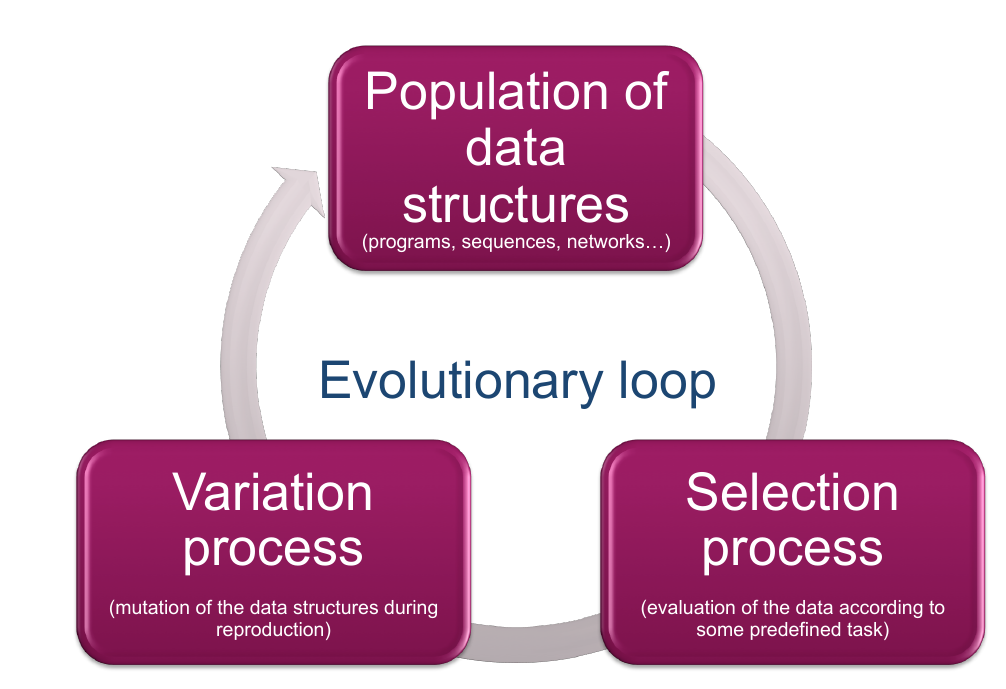
\includegraphics[width=0.8\textwidth]{figs/evol_loop}
\end{figure}
\end{frame}


\begin{frame}
 \frametitle{In-silico experimental evolution}
  \begin{figure}
        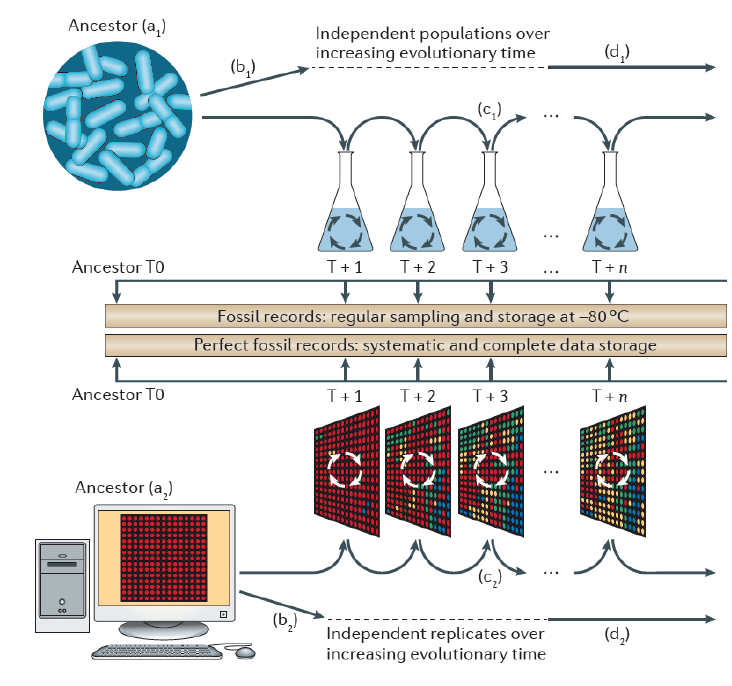
\includegraphics[width=0.6\textwidth]{figs/in_silico_evol}
\end{figure}
\end{frame}

\begin{frame}
 \frametitle{The biological model of Aevol}
  \begin{figure}
        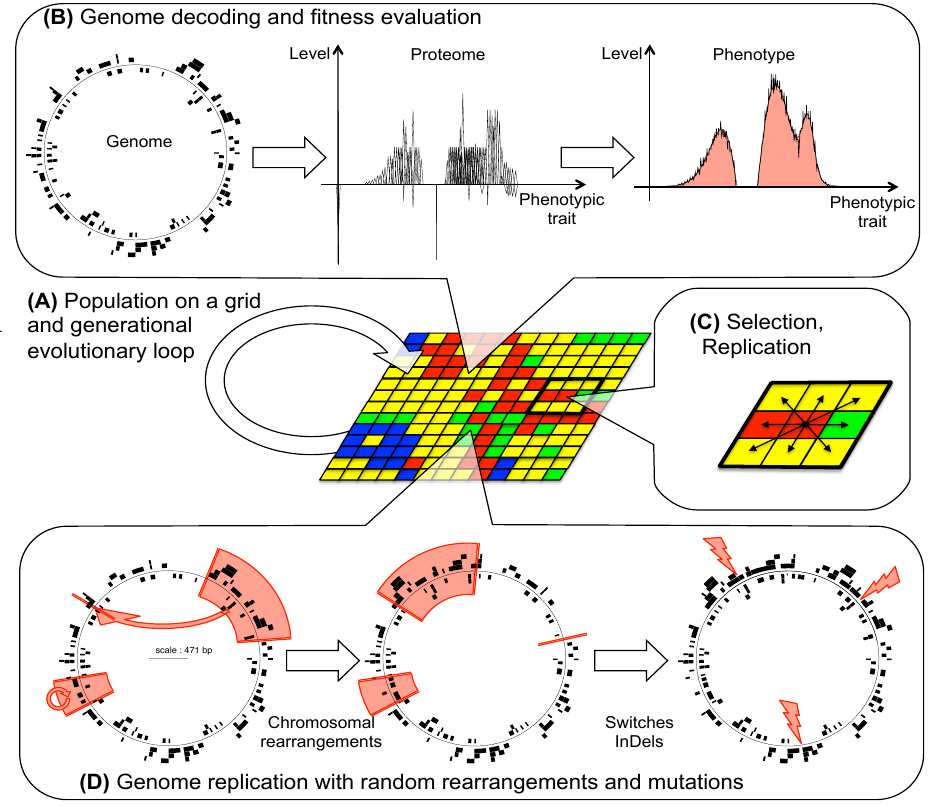
\includegraphics[width=0.7\textwidth]{figs/aevol}
\end{figure}
\end{frame}

\begin{frame}
 \frametitle{The biological model: A computer science view}
   \begin{figure}
   \only<1>{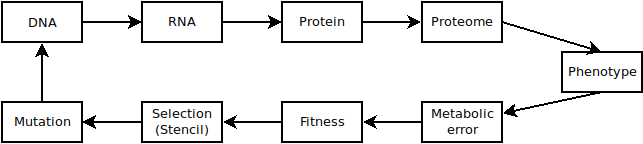
\includegraphics[width=0.7\textwidth]{figs/workflow}}
   \only<2>{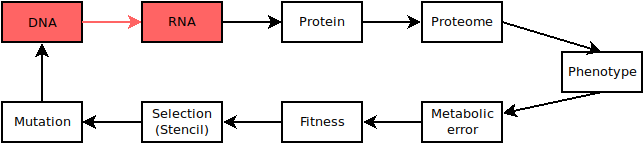
\includegraphics[width=0.7\textwidth]{figs/workflow_1}}
   \only<3>{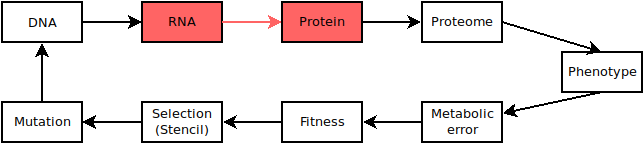
\includegraphics[width=0.7\textwidth]{figs/workflow_2}}
   \only<4>{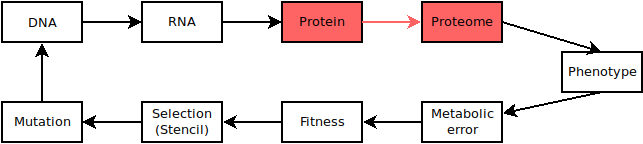
\includegraphics[width=0.7\textwidth]{figs/workflow_3}}
   \only<5>{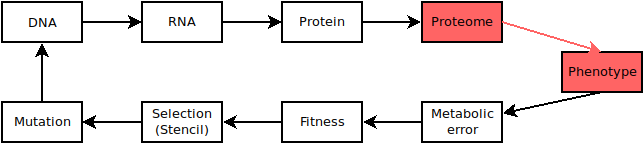
\includegraphics[width=0.7\textwidth]{figs/workflow_4}}
   \only<6>{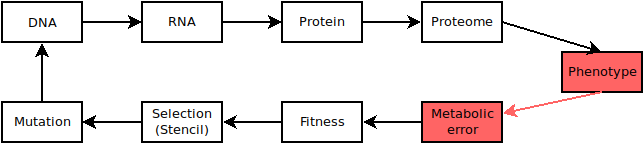
\includegraphics[width=0.7\textwidth]{figs/workflow_5}}
   \only<7>{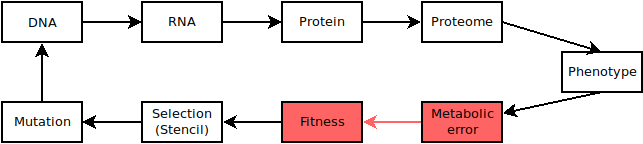
\includegraphics[width=0.7\textwidth]{figs/workflow_6}}
   \only<8>{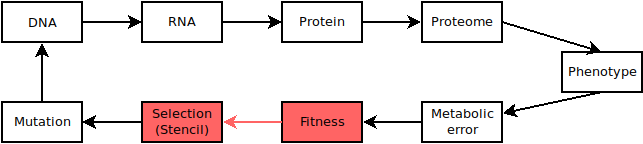
\includegraphics[width=0.7\textwidth]{figs/workflow_7}}
   \only<9>{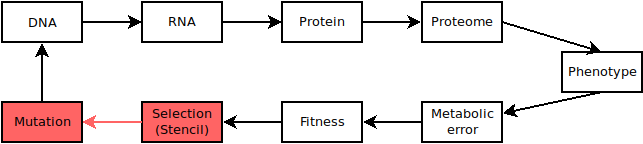
\includegraphics[width=0.7\textwidth]{figs/workflow_8}}
\end{figure}
\only<1>{
  \begin{itemize}
   \item The workflow is repeat for every cell of the grid
   \item Each cell contains one and only one organism
  \end{itemize}
}
 \only<2-6>{
 \begin{itemize}
  \item DNA $\rightarrow$ RNA : \textbf{Transcription} : Looking for 2 motifs
  \only<2>{
  \begin{enumerate}
   \item Promoter (size = 22) : Hamming distance (predefined motif, max. error = 4)
   \item Terminator (size = 4) : Exact match ($DNA[pos:pos+4]==DNA[pos+10:pos+14]$)
  \end{enumerate}
   }
   \only<3->{
  \item RNA $\rightarrow$ Protein : \textbf{Translation} : Looking for 2 motifs}
  \only<3>{
  \begin{enumerate}
   \item Shine Dalgarno (size = 6) + space (size = 4) + Start (size = 3) : Exact match
   \item Stop (size = 3) : Exact match
  \end{enumerate}
}
\only<4->{
  \item Protein $\rightarrow$ Proteome : \textbf{Folding} : }
  \only<4>{
  \begin{itemize}
  \item Looking for $N = \frac{Protein\_Length}{3}$ motifs
  \item Decoding each triple to addition to $M$, $W$, $H$ variables
  \item Translation $M$, $W$, $H$ into triangle and approx. them into $300$ double array
  \end{itemize}
  }
\only<5->{
  \item Proteome $\rightarrow$ Phenotype : \textbf{Summing arrays} : }
  \only<5>{
  \begin{itemize}
  \item Looking for $N = \frac{Protein\_Length}{3}$ motifs
  \item Decoding each triple to addition to $M$, $W$, $H$ variables
  \item Translation $M$, $W$, $H$ into triangle and approx. them into $300$ double array
   \item Summing into a global $300$ double array
  \end{itemize}
  }
  \only<6->{
  \item Phenotype $\rightarrow$ Metabolic error: \textbf{Difference betwen 2 arrays}
 \only<6>{
 \begin{itemize}
   \item Phenotypical Target : Pre-defined array built from a sum of gaussians
   \item Compute the difference the Phenotype and the phenotypical target
  \end{itemize}
  }
}
 \end{itemize}
 }
 \only<7->{
 \begin{itemize}
  \item Metabolic error $\rightarrow$ Fitness:
  \only<7>{
  \begin{itemize}
   \item $exp(-selection\_pressure \times metabolic\_error)$
  \end{itemize}
  }
  \only<8->{
  \item Fitness $\rightarrow$ Selection : \textbf{Stencil 9-point 2D}
  \only<8>{
  \begin{itemize}
   \item Only kernel requiring data coming from other cells of the grid
   \item Fetch fitness of the neighboring cells
   \item Use the fitness proportionate algorithms to select the organism that will reproduce in the cell
   \item Delete the old organism
    \item Copy the DNA of the organism into the cell
  \end{itemize}
  }
  }
  \only<9->{
  \item Selection $\rightarrow$ Mutation : \textbf{Modify the DNA}
  \only<9>{
  \begin{itemize}
   \item Switch of the value of up to 6 value in the DNA array
  \end{itemize}
  }
  }
 \end{itemize}
 }
 
\end{frame}

\begin{frame}
 \frametitle{Aevol VS mini-Aevol}
 \begin{itemize}
  \item Aevol VS micro-Aevol SLOC : 87,000 VS 2,800 
  \vfill
  \item Simplify model
  \begin{itemize}
  \item Only a strand of DNA (and not too) \textit{i.e.} the DNA is read one-way and not both-way
  \item A reduce mutation sets: no mutation that change the size
  \item A lot of advances features are missing: no plasmid, 4bp DNA, ...
  \end{itemize}
  \vfill
  \item Implementation
  \begin{itemize}
   \item Lot less robust to input errors
   \item Can not change model parameters during an evolution
   \item No phylogenetic tree
   \item No postprocessing tool
  \end{itemize}
 \end{itemize}
\end{frame}

% \begin{frame}
%  \frametitle{The R- version (Aevol and mini-Aevol)}
% \end{frame}

% \section{Implementation}
% \begin{frame}
%  \frametitle{Implementation}
%  
% \end{frame}

\section{Optimizations}
\begin{frame}
 \frametitle{Optimizations}
 \begin{itemize}
  \item Working only on diff (where the DNA has changed during the mutation) \textit{i.e.} do not reparse the whole DNA at each generation (available in the git repository for sequential CPU)
  \item Remove the modulo that allows to simulate circular DNA (copy a part of the beginning of the DNA at the end to do it)
  \item Change the coding of the DNA from a char array to a bitset
  \item Vectorization of the comparison between DNA and motifs
  \item Search multiple motifs at once through vectorization
  \item Evaluate classic mutation operator (malloc+memcpy+mutation) and backtrace mutation operator (malloc+copy)
  \item One large 1D structure (merge all DNAs into a big DNA) to ease load balancing
  \item Include metadata (promoter, terminator, start, stop) into a bitset
 \end{itemize}
\end{frame}

\section{Parallelization}
\begin{frame}
 \frametitle{Parallelization}
 \begin{itemize}
  \item OpenMP (parallel for and/or tasks with or without dependency)
  \item CUDA
  \item OpenACC
  \item MPI
  \item Hybrid \textit{e.g.} OpenMP+OpenACC, OpenMP+MPI, ...
  \vfill
  \item Implement the stencil (\textit{i.e.} asynchronous time between grid cells)
 \end{itemize}
\end{frame}


\section{Methodology}
\begin{frame}
 \frametitle{Methodology}
\begin{enumerate}
 \item Use GIT (or another versioning software)
 \item For each optimization/parallelization, tests its performance, scalability (weak and strong) and create visualization of them
 \item You need to verify the reproduceability of your code \textit{i.e.}, same parameters must lead to same results
\end{enumerate}
\vfill
Simulation parameters:
\begin{itemize}
 \item Size of the DNA ($-g$): 500, 5000, 50,000 (you can go up to 500,000)
 \item Population size ($-w$ and $-h$) : 32x32, 128x128, 256x256 (you can up to 1024x1024)
 \item Mutation rate ($-m$) : 0.0001, 0.00001, 0.000001
\end{itemize}


 \end{frame}




\end{document}
